\section{Cavity with a defect}
\label{sec:defect_cavity}
The first new geometry explored is a cavity with a defect. This is a cavity with geometry very similar to the one described in section \ref{sec:simple_cavity}, except that the helix is "broken" exactly at the centre of the cavity. This means the cavity is modelled by two identical chiral media, one of which as a start angle different from the other. This geometry is schematized in figure \ref{fig:defect}.

\subsection{Reflectivities}

As with the first cavity, the passive reflectivity is examined. This cavity is expected to behave as a very selective filter. Figure \ref{fig:defect_reflectivity} shows three reflectivity plots of right-handed cavities. The simplest is probably the first one, \ref{fig:defect_reflectivity:reflect}, with a $\frac{\pi}{2}$ defect and no losses. The narrow band filter behaviour is present at the Bragg wavelength, \textit{i.e.} $\Re{\bar{n}}\times L_p$\cite{mccall_simplified_2009}. Then, \ref{fig:defect_reflectivity:reflect_losses} shows that the introduction of losses in the medium decreases the filtering efficiency. Finally, by varying the angle of the defect, it is possible to tune the zero-reflectivity wavelength, as shown in figure \ref{fig:defect_reflectivity:reflect_other}. The transmitivities were also calculated, but do not show any remarkable feature that is not already displayed by reflectivities. Transmitivities are shown in appendix \ref{chap:transmitivities}.

\begin{figure}
	\centering
	\begin{subfigure}{0.49\linewidth}
		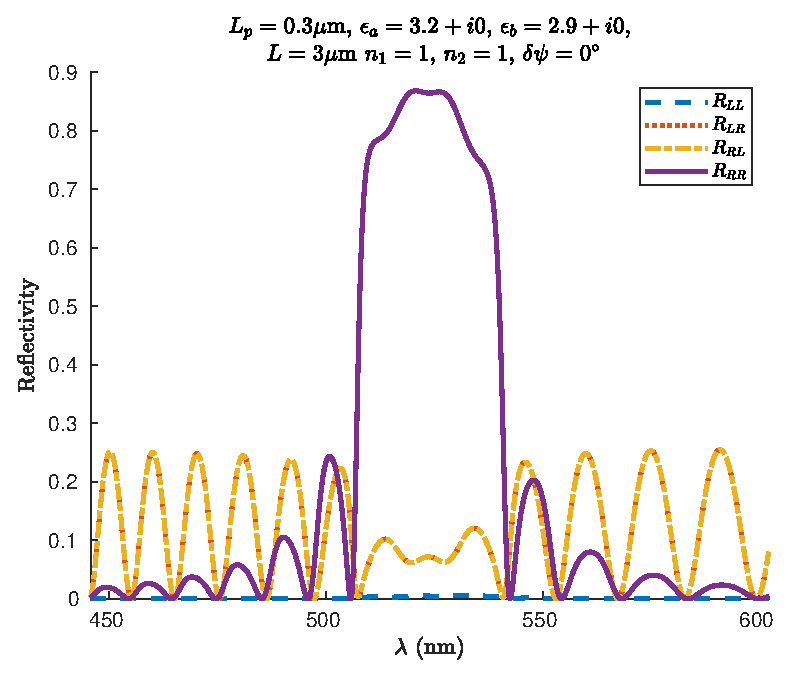
\includegraphics[width=\linewidth]{plots/defect/no_defect/oseen_reflection}
		\caption{}
		\label{fig:defect_reflectivity:reflect_nodefect}
	\end{subfigure}
	\begin{subfigure}{0.49\linewidth}
		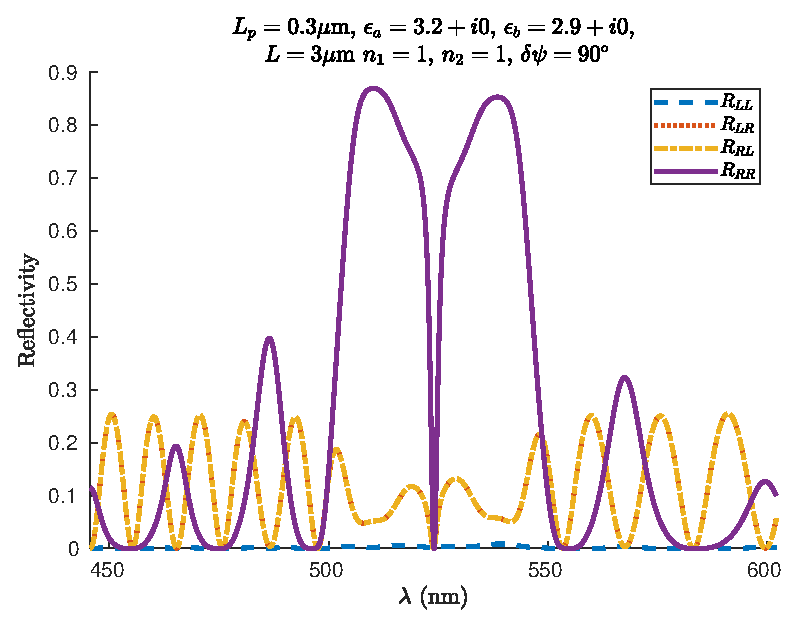
\includegraphics[width=\linewidth]{plots/defect/reflectivity/oseen_reflection}
		\caption{}
		\label{fig:defect_reflectivity:reflect}
	\end{subfigure}
	\begin{subfigure}{0.49\linewidth}
		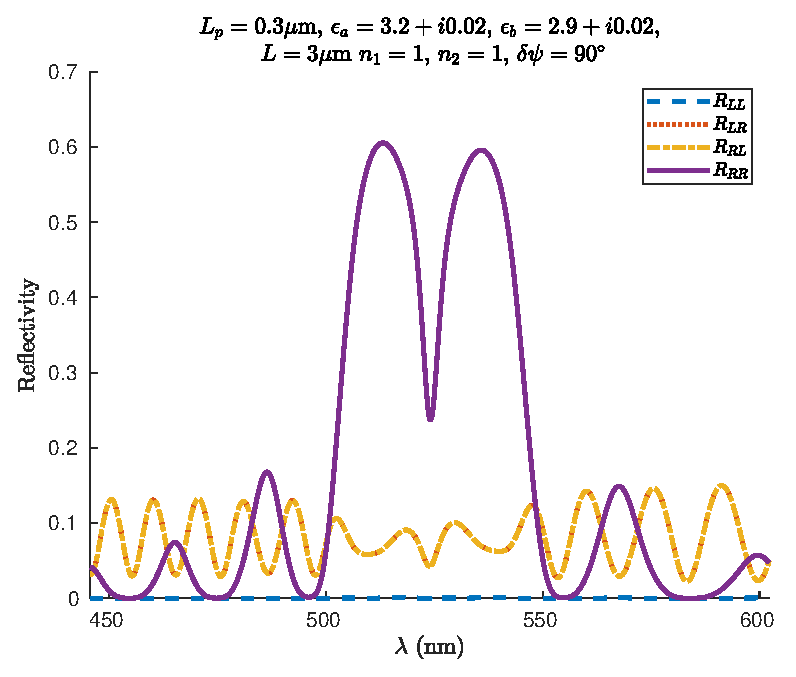
\includegraphics[width=\linewidth]{plots/defect/reflectivity_losses/oseen_reflection}
		\caption{}
		\label{fig:defect_reflectivity:reflect_losses}
	\end{subfigure}
	\begin{subfigure}{0.49\linewidth}
		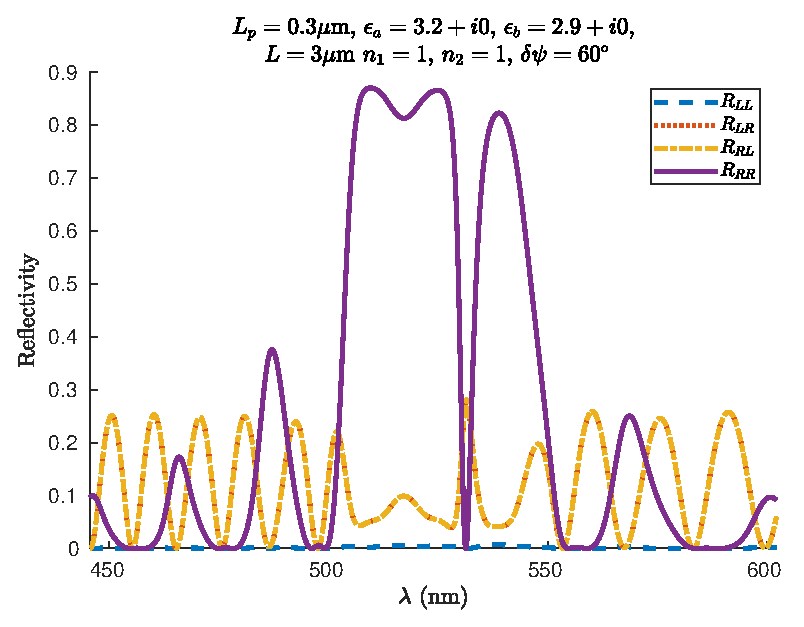
\includegraphics[width=\linewidth]{plots/defect/reflectivity_other_defect/oseen_reflection}
		\caption{}
		\label{fig:defect_reflectivity:reflect_other}
	\end{subfigure}
	\caption[Reflectivity of the narrow-band filter]{Reflectivities calculated for a right-handed cavity with a defect with the exact theory. Parameters are given on each figure. The results obtained with coupled wave theory are very close and a comparison is available in figures \ref{fig:reflectivities_narrow_appendix} and \ref{fig:reflectivities_narrow_appendix_comp} in appendix \ref{chap:reflectivities}. \ref{fig:defect_reflectivity:reflect_nodefect} Reflectivity without defect and without losses. \ref{fig:defect_reflectivity:reflect} Reflectivity for a defect of $\pi/2$ without losses. \ref{fig:defect_reflectivity:reflect_losses} Reflectivity for a defect of $\pi/2$ with losses. \ref{fig:defect_reflectivity:reflect_other} Reflectivity for a defect of $\pi/3$ without losses.}
	\label{fig:defect_reflectivity}
\end{figure}

\subsection{Laser action}

With the same methodology as before, lasing action is examined in the defect cavity. Figure \ref{fig:defect_cavity:surf} shows the positions of laser modes found for a cavity parametrised by table \ref{tab:defect_cavity:simulation}. The exact and approximate theories yield similar results.

\begin{table}
	\centering
	\begin{tabulary}{\linewidth}{LCC}
		\hline
		\hline
		Structural period of the chiral medium & $L_p$ & 300 nm \\
		Length of the chiral medium & $L$ & $2\times10\times L_p$ \\
		Refractive index of the surrounding media & $n_1=n_2$ & 1 \\
		Average refractive index of the chiral medium (Re) & $\bar{n}$ & 1.7690 \\
		Detuning range & $\mathrm{Re}(\delta k L / 2)$ & $[0,5]$ \\
		Gain range & $-\mathrm{Im}(\delta k L / 2)$ & $[0,1.2]$ \\
		Coupling constant & $\kappa$ & $4/L$ \\
		Defect & $\psi$ & $\frac{\pi}{2}$\\
		\hline
		\hline
	\end{tabulary}
	\caption[Parameters for the cavity with a defect]{Parameters used for simulation.}
	\label{tab:defect_cavity:simulation}
\end{table}

Figure \ref{fig:defect_cavity:modes_found} displays the corresponding output modes. This shows the modes outputted by this laser are still un-pure. However, the hypothesis on the strong confinement of right-handed polarised light turns out to be verified. Indeed, figure \ref{fig:defect_cavity:intensity_distribution} shows that mode 2 provides such a confinement.

It was also found that the angle of the defect was a handful way of tuning the cavity. Indeed, by changing the angle of the second slab of chiral medium, a whole range of lasing modes was made available. This is shown in figure \ref{fig:defect_cavity:tuning}. An animation is also available at \url{http://klafyvel.me/lasing_coeff_defect.avi}.
\begin{wrapfigure}{r}{0.30\textwidth} %this figure will be at the right
	\capstart
	\centering
	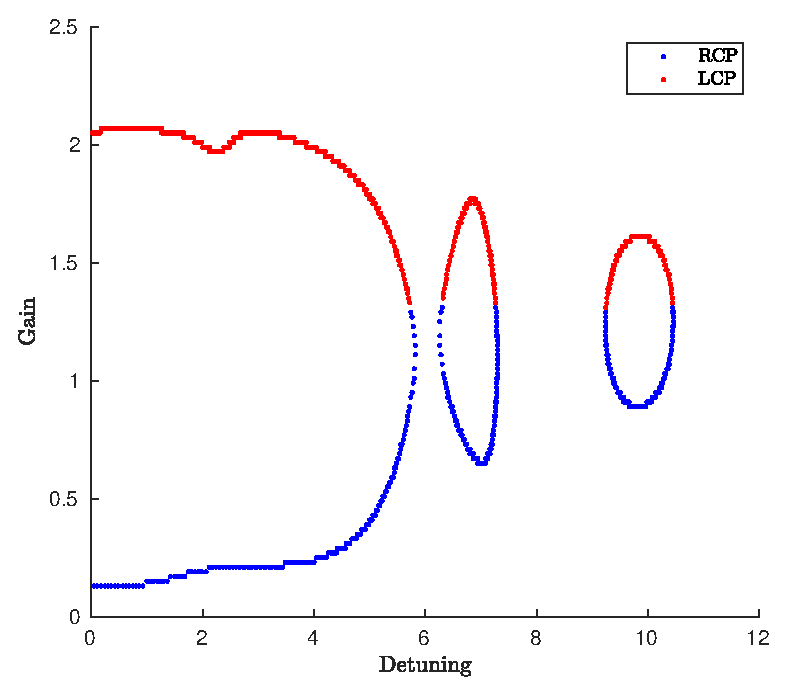
\includegraphics[width=0.30\textwidth]{plots/defect/tuning}
	\caption[Tuning of defect cavity]{Tuning of defect cavity. Modes are identified according to their handedness (\protect\tikz[baseline=-0.5ex]{\protect\fill[color=red] (0,0) circle (1ex) ;} left-handed, \protect\tikz[baseline=-0.5ex]{\protect\fill[color=blue] (0,0) circle (1ex) ;} right-handed) for a range of defect angle of $[-\pi;\pi]$}
	\label{fig:defect_cavity:tuning}
\end{wrapfigure}

\begin{figure}
	\centering
	\begin{subfigure}{0.49\textwidth}
		\begin{subfigure}{\textwidth}
			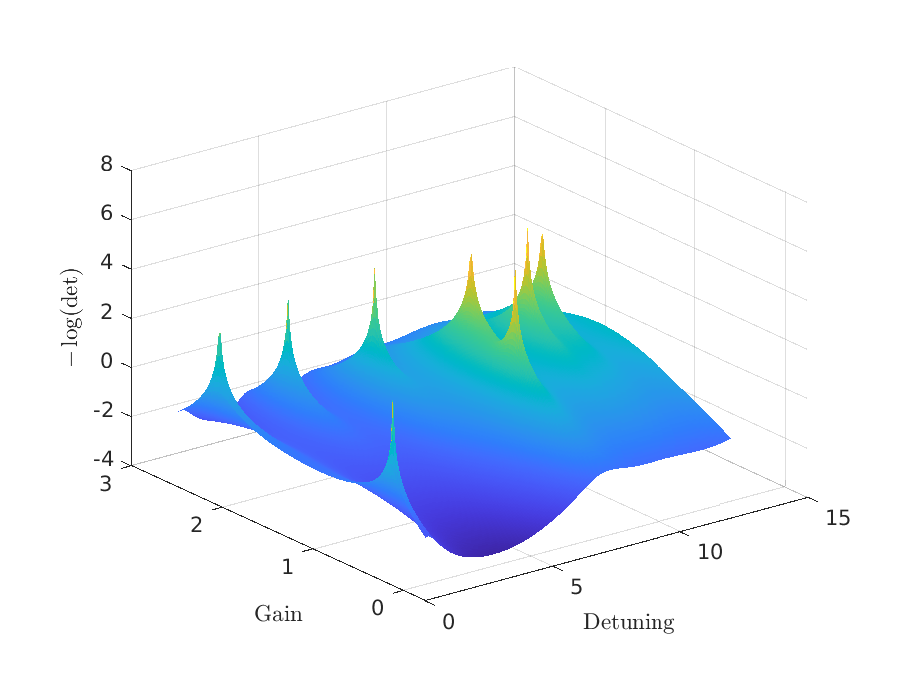
\includegraphics[width=\textwidth]{plots/defect/surface_oseen}
			\caption{}
			\label{fig:defect_cavity:oseen_surf}
		\end{subfigure}
		\begin{subfigure}{\textwidth}
			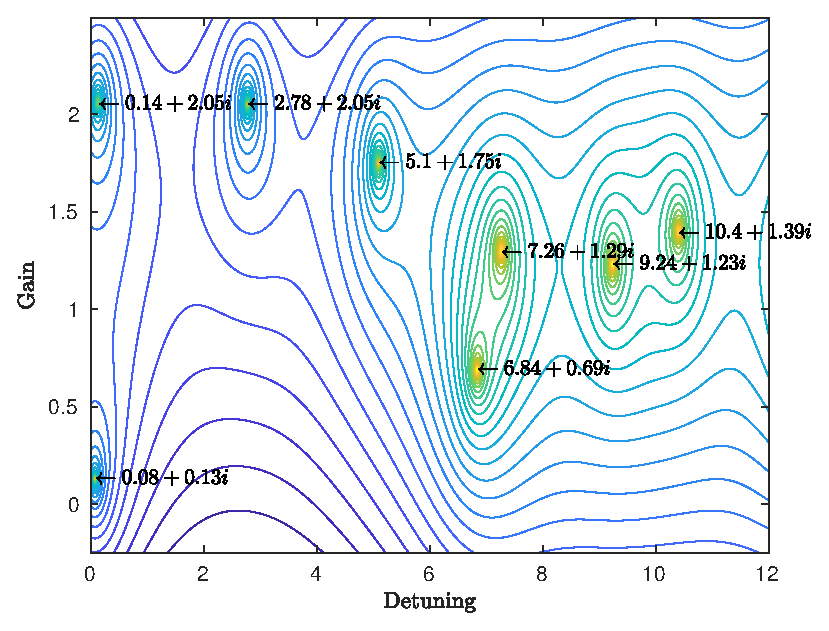
\includegraphics[width=\textwidth]{plots/defect/contour_oseen}
			\caption{}
			\label{fig:defect_cavity:oseen_contour}
		\end{subfigure}
		\begin{subfigure}{\textwidth}
			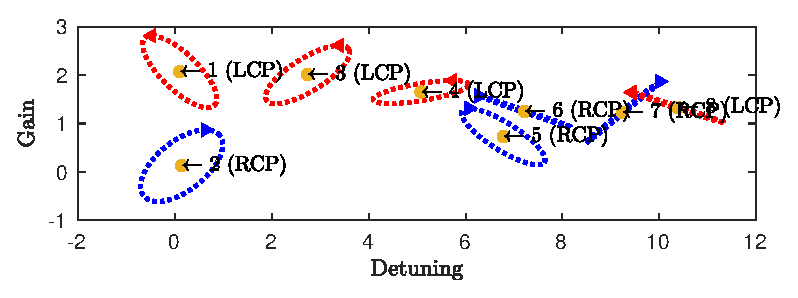
\includegraphics[width=\textwidth]{plots/defect/modes_found}
			\caption{}
			\label{fig:defect_cavity:modes_found}
		\end{subfigure}
	\end{subfigure}
	\begin{subfigure}{0.49\textwidth}
		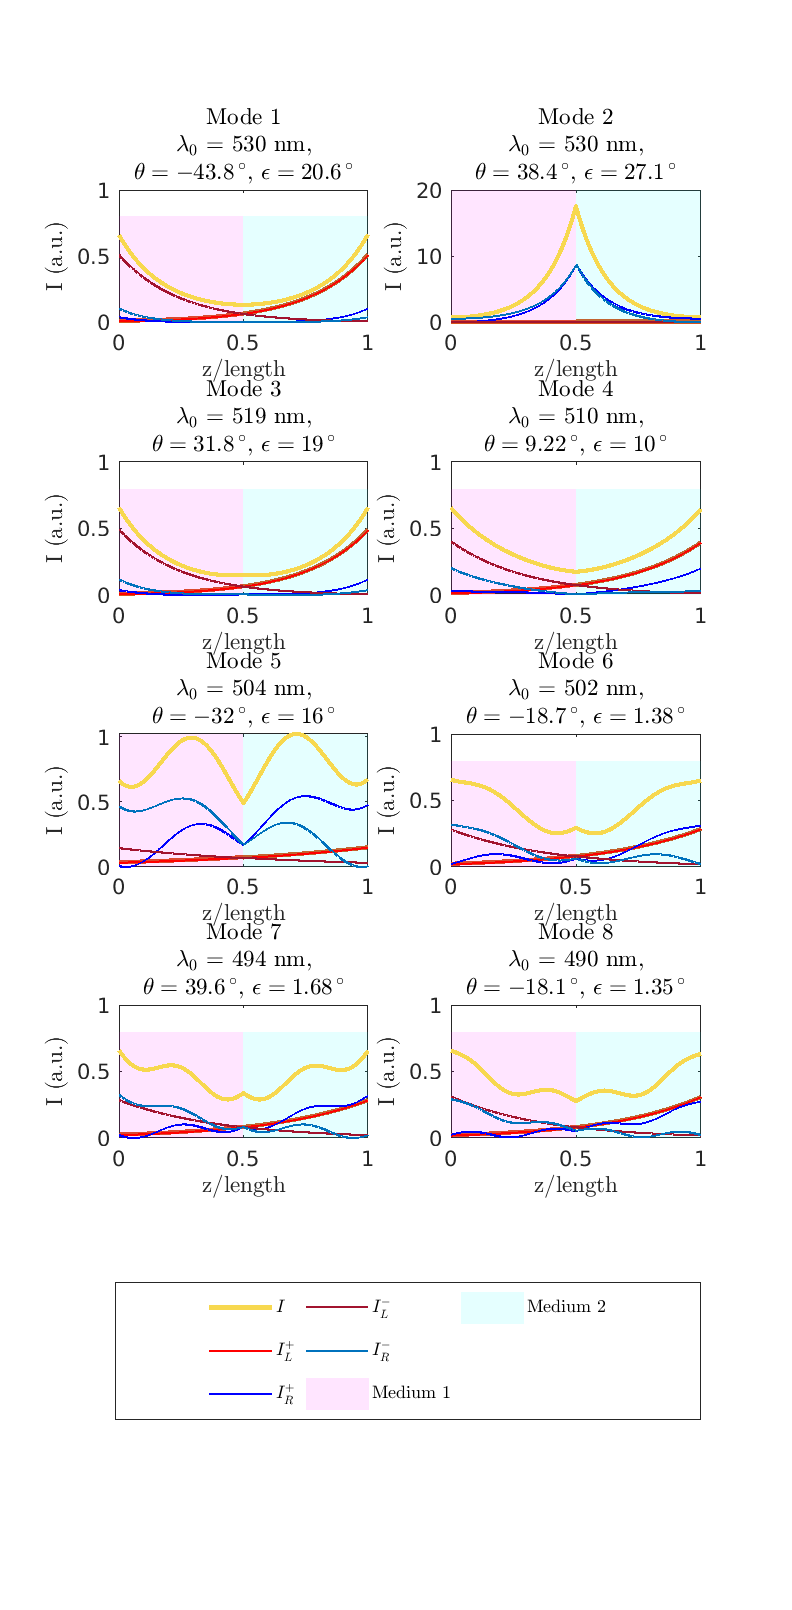
\includegraphics[width=\textwidth]{plots/defect/intensity_distribution}
		\caption{}
		\label{fig:defect_cavity:intensity_distribution}
	\end{subfigure}
	\caption[Comparison between methods for modeling a defect cavity.]{Analysis of the defect cavity. \ref{fig:defect_cavity:oseen_surf} shows the logarithm of the invert of the determinant of $\bm{M_{22}}$. \ref{fig:defect_cavity:oseen_contour} is the corresponding contour plot where the lasing modes have been identified. \ref{fig:defect_cavity:modes_found} Labeled modes found with the developed CWT and corresponding output ellipses in medium 1. \ref{fig:defect_cavity:intensity_distribution} Intensity distribution in the cavity for the modes in \ref{fig:defect_cavity:modes_found}. The intensity distribution yielded by exact theory is close to the approximate result and is given in figure \ref{fig:defect_intensity_appendix} in appendix \ref{chap:intensities}.}
	\label{fig:defect_cavity:surf}
\end{figure}

\subsection{Conclusion on the cavity with a defect}
	
This geometry does not produce pure circularly-polarised light. However it allows for interesting features such as highly selective band filter and fine laser tuning. The benefits of this cavity could be adapted in future designs in conjunction with a design allowing the output of purer circular modes.